\section{Anwendungsfälle}
Aus den in Kapitel \ref{chap:szenarien} erarbeiteten Szenarien ergeben sich die folgenden Use-Cases, die von einer offlinefähigen Anwendung erfüllt werden sollen. Die folgende Tabelle zeigt die Anwendungsfälle aus der Entwicklungsperspektive.
\begin{longtable}[c]{@{}
>{\columncolor[HTML]{CFFCC2}}l ll@{}}
\toprule
    \multicolumn{1}{p{0.1\textwidth}}{\cellcolor[HTML]{cffcc2}\textbf{ID}}
    & \multicolumn{1}{p{0.45\textwidth}}{\cellcolor[HTML]{cffcc2}\textbf{Anwendungsfall}}
    & \multicolumn{1}{p{0.45\textwidth}}{\cellcolor[HTML]{cffcc2}\textbf{Beschreibung}}\\ \hline
\endfirsthead
%
\endhead
%
  \multicolumn{1}{l}{\cellcolor[HTML]{cffcc2}\textbf{UC1}} &
  \multicolumn{1}{p{0.45\textwidth}}
  {Um die Anwendung auch ohne Internetzugang zu nutzen, sollen die Daten auch offline erreichbar sein.}
  & \multicolumn{1}{p{0.45\textwidth}}
  {Die Daten werden auf dem Server und lokal gespeichert. Lokal bedeutet in einer lokalen Datenbank oder im Browser (localStorage, IndexedDB usw.)}.\\
  \midrule
  % UC2
  \multicolumn{1}{l}{\cellcolor[HTML]{cffcc2}\textbf{UC2}} & \multicolumn{1}{p{0.45\textwidth}}
  {Um Datentraffic und Ladezeiten zu sparen möchte ich nur die Adressbucheinträge oder deren Aktualisierungen laden, die sich nicht schon auf dem Endgerät befinden.}
  & \multicolumn{1}{p{0.45\textwidth}}
  {Es wird ermittelt welche Daten neu angelegt oder aktualisiert wurden. Dazu müssen sie sortierbar und versionierbar sein.}\\
  \midrule
  % UC3
  \multicolumn{1}{l}{\cellcolor[HTML]{cffcc2}\textbf{UC3}} & \multicolumn{1}{p{0.45\textwidth}}
  {Um jedem Adressbucheintrag Operationen zuzuweisen, möchte ich die Einträge identifizieren.}
  & \multicolumn{1}{p{0.45\textwidth}}
  {Jeder Eintrag bekommt zur eindeutigen Identifikation eine \gls{UUID} zugewiesen.}\\
  \midrule
  % UC4
  \multicolumn{1}{l}{\cellcolor[HTML]{cffcc2}\textbf{UC4}} & \multicolumn{1}{p{0.45\textwidth}}
  {Um zu wissen ob, wie oft und wann ein Eintrag aktualisiert wurde, möchte ich die Einträge versionieren.}
  & \multicolumn{1}{p{0.45\textwidth}}
  {Jeder Eintrag bekommt ein Versionsattribut.}\\
  \midrule
  % UC5
  \multicolumn{1}{l}{\cellcolor[HTML]{cffcc2}\textbf{UC5}} & \multicolumn{1}{p{0.45\textwidth}}
  {Um sicherzustellen, dass keine Daten verloren gehen, soll mit Konflikten umgegangen werden.}
  & \multicolumn{1}{p{0.45\textwidth}}
  {\todo{Jeder Konflikt wird (in der Versionsliste) gespeichert und kann so auch manuell gelöst werden.}}\\
  \midrule
  % UC6
  \multicolumn{1}{l}{\cellcolor[HTML]{cffcc2}\textbf{UC6}} &
  \multicolumn{1}{p{0.45\textwidth}}
  {Um sicherzustellen, dass keine Daten verloren gehen, soll mit Konflikten umgegangen werden.}
  &
  \multicolumn{1}{p{0.45\textwidth}}
  {\todo{Jeder Konflikt wird (in der Versionsliste) gespeichert und kann so auch manuell gelöst werden.}}\\
  \midrule
  % UC7
  \multicolumn{1}{l}{\cellcolor[HTML]{cffcc2}\textbf{UC7}} & \multicolumn{1}{p{0.45\textwidth}}
  {Um sicherzustellen, dass keine Daten verloren gehen, soll mit Konflikten umgegangen werden.}
  & \multicolumn{1}{p{0.45\textwidth}}
  {\todo{Jeder Konflikt wird (in der Versionsliste) gespeichert und kann so auch manuell gelöst werden.}}\\
  % end
  \bottomrule \cellcolor[HTML]{FFFFFF}
  \vspace{0.1cm}\\
  \noalign{\hspace{0.0525\textwidth}\grayRule}
  \caption{Anwendungsfälle}
  \label{tab:uc}\\
\end{longtable}

Das in Abbildung \ref{fig:uc} gezeigte Use-Case-Diagramm veranschaulicht die in der obigen Tabelle \ref{tab:uc} aufgeführten Anwendungsfälle.
\begin{figure}[H]
    \centering
    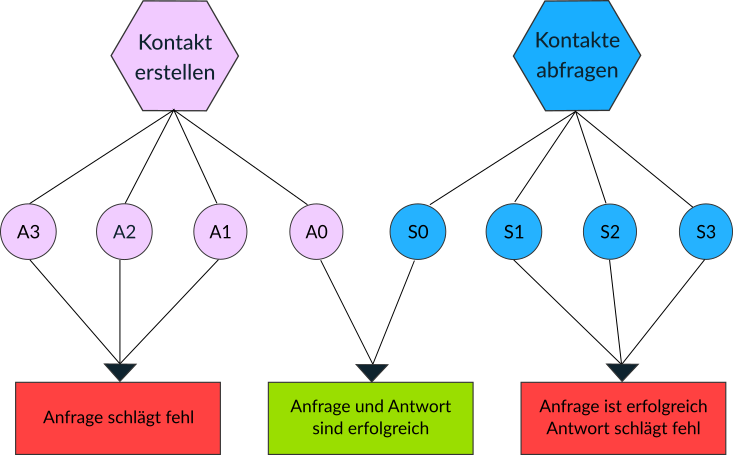
\includegraphics[width=\textwidth]{Szenarien}
    \grayRule
    \caption{Use-Case-Diagramm}
    \label{fig:uc}
\end{figure}